\documentclass{abntex2}
\usepackage[utf8]{inputenc}
\usepackage{graphicx}
\usepackage[num]{abntex2cite}

\titulo{Experimento 2: Regulador de tensão}
\autor{Lucas Rezende de Macedo - 14/0026363\\Jônatas Ribeiro Senna Pires - 14/0090983}
\data{9 de Abril de 2018}
\local{Brasília, Distrito Federal}

\begin{document}

\imprimircapa
\imprimirfolhaderosto

\tableofcontents
\listoffigures
\clearpage

\chapter{Experiências}

O procedimento experimental consiste na verificação do funcionamento dos circuitos retificadores representados pelas figuras \ref{fig:circuito1} e \ref{fig:circuito2}.

\begin{figure}[h]
  \centering
  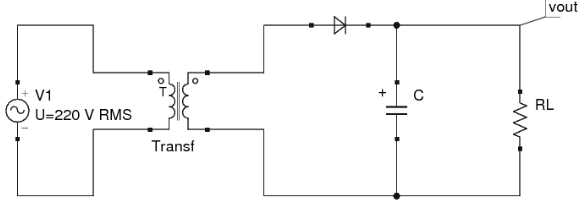
\includegraphics[scale = 0.7]{circuito1.png}
  \caption{Circuito retificador de meia onda montado no procedimento experimental.}
  \label{fig:circuito1}
\end{figure}

\begin{figure}[h]
  \centering
  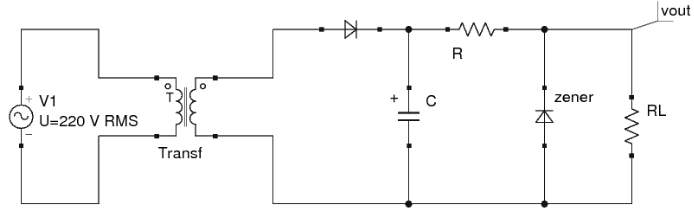
\includegraphics[scale = 0.7]{circuito2.png}
  \caption{Circuito retificador de meia onda com regulação de tensão por diodo zener montado no procedimento experimental.}
  \label{fig:circuito2}
\end{figure}

\section{Experiência 1}

Para a primeira montagem do circuito da figura \ref{fig:circuito1}, sem a carga ($R_L$), temos que a entrada ($v_I$) e saída no capacitor ($v_o$) são definidas conforme a figura \ref{fig:io1}.
\pagebreak

\begin{figure}[h]
  \centering
  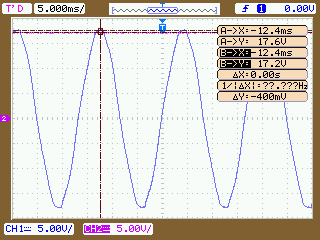
\includegraphics[scale = 0.7]{exp1-1.png}
  \caption{Gráfico da entrada (azul) e saída (rosa) do circuito da figura \ref{fig:circuito1} sem a carga ($R_L$).}
  \label{fig:io1}
\end{figure}

Para a segunda montagem do circuito da figura \ref{fig:circuito1}, com a carga ($R_L) = 2.17 k\Omega$, temos que a entrada ($v_I$) e saída no capacitor ($v_o$) são definidas conforme a figura \ref{fig:io2}.

\begin{figure}[h]
  \centering
  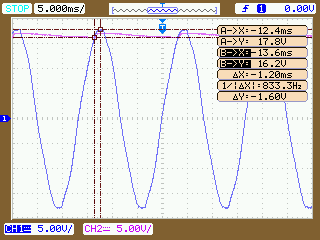
\includegraphics[scale = 0.7]{exp1-2.png}
  \caption{Gráfico da entrada (azul) e saída (rosa) do circuito da figura \ref{fig:circuito1} com a carga ($R_L$).}
  \label{fig:io2}
\end{figure}

\pagebreak
\section{Experiência 2}

Para o circuito da figura \ref{fig:circuito2}, realizamos a montagem com um resistor $R = 992.3\Omega$ com o capacitor $C = 1000\mu F$, $25V$. Para cada valor de resistência de carga ($R_L$) medimos os valores de tensão presentes na tabela \ref{tab:tensoes}.

Para obter a resistência de carga ($R_L = 492.15\Omega$) utilizamos dois resistores de resitência nominal $1k\Omega$ em paralelo. De forma análoga, para obter a resistência de carga ($R_L = 315.3\Omega$), utilizamos um resistor de $100\Omega$ e um de $220\Omega$ em série.

As tensões no capacitor e na carga para os valore de $R_L$ podem ser verificados nos gráficos das figuras \ref{fig:graf1} a \ref{fig:graf5}

\begin{table}[h]
\centering
\begin{tabular}{|l|l|l|l|l|}
\hline
$R_L(\Omega)$ & $V_{DC}$(V) & $V_{DC}(\infty) - V_{DC}(R_L)$ (V) & $V_{PP}^C$ (mV) & $V_{PP}^{R_L}$ (mV) \\
\hline
\infty        & 8,74      & 0                              & 146             & 10                  \\
\hline
2,17k         & 8,67      & 0,07                           & 150             & 10                  \\
\hline
985           & 8,33      & 0,41                           & 156             & 76                  \\
\hline
492,15        & 5,48      & 3,26                           & 206             & 66                  \\
\hline
315,3         & 3,96      & 4,78                           & 230             & 58                  \\
\hline
\end{tabular}
\label{tab:tensoes}
\caption{Tabela de valores de tensão para cada valor de $R_L$.}
\end{table}

\begin{figure}[h]
  \centering
  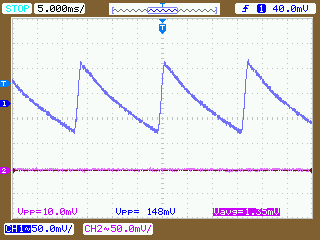
\includegraphics[scale = 0.7]{exp2-1.png}
  \caption{Gráfico da tensão no capacitor (azul) e na saída (rosa) do circuito da figura \ref{fig:circuito2} com a carga ($R_L = \infty$).}
  \label{fig:graf1}
\end{figure}

\begin{figure}[h]
  \centering
  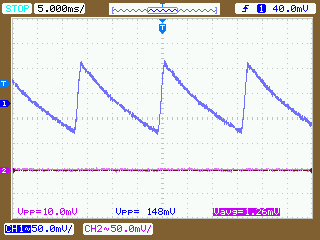
\includegraphics[scale = 0.7]{exp2-2.png}
  \caption{Gráfico da tensão no capacitor (azul) e na saída (rosa) do circuito da figura \ref{fig:circuito2} com a carga ($R_L = 2,17k\Omega$).}
  \label{fig:graf2}
\end{figure}

\begin{figure}[h]
  \centering
  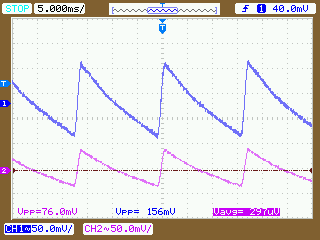
\includegraphics[scale = 0.7]{exp2-3.png}
  \caption{Gráfico da tensão no capacitor (azul) e na saída (rosa) do circuito da figura \ref{fig:circuito2} com a carga ($R_L = 985\Omega$).}
  \label{fig:graf3}
\end{figure}

\begin{figure}[h]
  \centering
  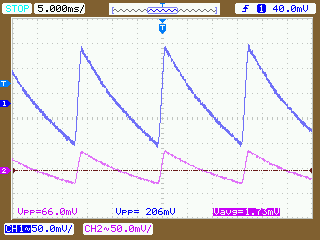
\includegraphics[scale = 0.7]{exp2-4.png}
  \caption{Gráfico da tensão no capacitor (azul) e na saída (rosa) do circuito da figura \ref{fig:circuito2} com a carga ($R_L = 492.15\Omega$).}
  \label{fig:graf4}
\end{figure}

\begin{figure}[h]
  \centering
  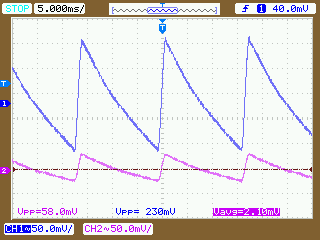
\includegraphics[scale = 0.7]{exp2-5.png}
  \caption{Gráfico da tensão no capacitor (azul) e na saída (rosa) do circuito da figura \ref{fig:circuito2} com a carga ($R_L = 315.3\Omega$).}
  \label{fig:graf5}
\end{figure}
\pagebreak
\chapter{Discussão}

\section{Questão 1 - Comportamento com a redução de $R_L$}

\section{Questão 2 - Comparação com o funcionamento de um retificador de onda completa}

% O periodo de ripple eh menor pq a frequencia dobra e o ripple diminui
Se o circuito montado fosse um retificador de onda completa, teríamos o esquemático mostrado na figura \ref{fig:retComp}.

\begin{figure}[h]
  \centering
  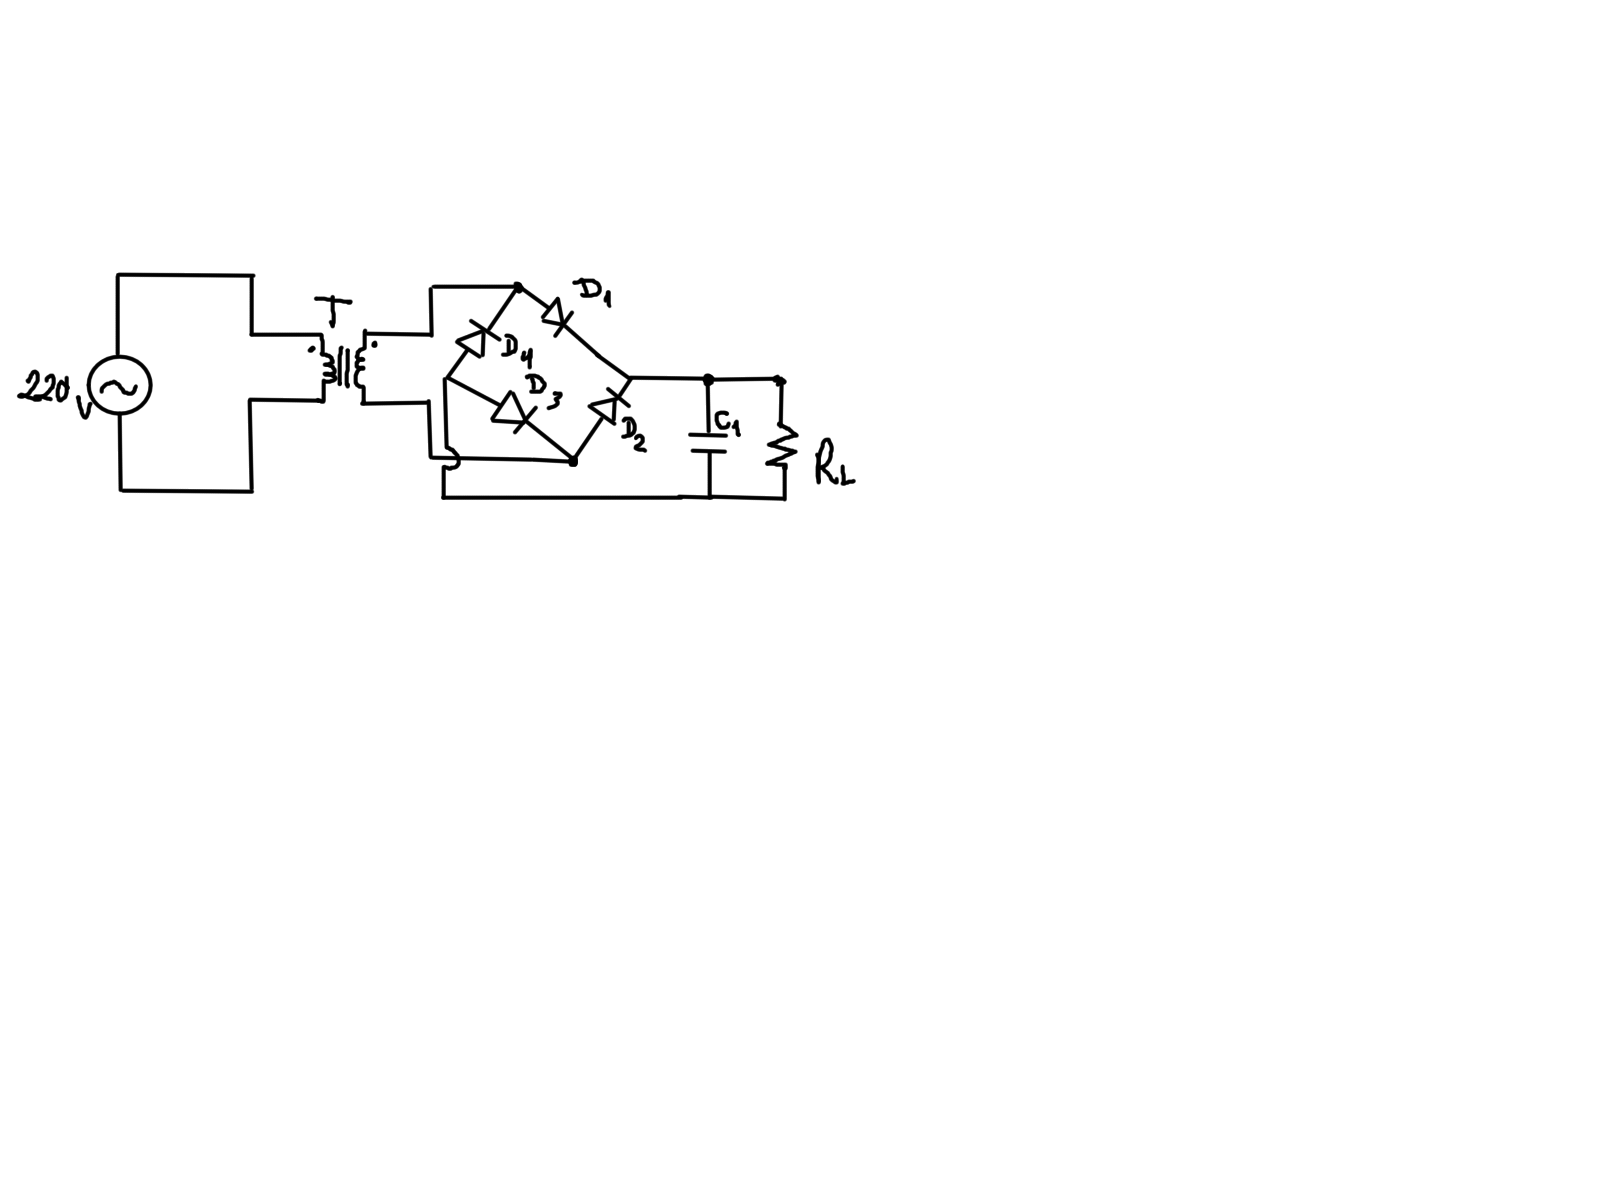
\includegraphics[scale = .7]{retComp.png}
  \caption{Esboço do circuito de um retificador completo com carga $R_L$.}
  \label{fig:retComp}
\end{figure}

O retificador de onda completa funciona de forma a aproveitar os momentos em que a onda de entrada está negativa. Ao analisar a equação (equação  \ref{eq:retComp}) que define Vripple para um retificador de onda completa é possível
chegar a algumas conclusões.
\begin{equation}
  V_r_i_p_p_l_e = \frac{V-2V_d^o^n}{RC2f_i_n}
  \label{eq:retComp}
\end{equation}

\begin{itemize}
  \item $V_r_i_p_p_l_e$ vai diminuir pela metade porque a frequência dobrou;
  \item $V_r_i_p_p_l_e$ Vai diminuir pois é reduzido de mais uma queda de tensão relacionada aos diodos adicionados;
  \item A frequência de $V_r_i_p_p_l_e$ vai dobrar por causa do aumento da frequência do sinal de entrada.
\end{itemize}

Como $V_r_i_p_p_l_e$ é um efeito indesejado, se fosse trocado um circuito retificador de meia onda por um circuito retificador de onda completa,
seria obtido um resultado final com $V_r_i_p_p_l_e$ menor, obtendo, assim, um resultado de saída com maior precisão.

\section*{Referências}


[1] SEDRA, Adel S.; SMITH, Kenneth Carless. Microelectronic circuits. New York: Oxford University Press, 1998.

[2] RAZAVI, Behzad; BEHZAD, Razavi. RF microelectronics. New Jersey: Prentice Hall, 1998.

\end{document}
